% !TEX root = ../disertace.tex
%!TEX encoding = UTF-8 Unicode

\chapter{\sdata}
\section{The design and the PML schema}
\sdata\ means s-layer PML files and the PML schema of these files. The idea behind \sdata\ design is to have a simple way to store additional ``sense'' annotations over any layer of PDT. The annotations are stored as a set of ``sense'' nodes. Each s-node contains a link to a sense repository (annotation lexicon) and a set of references to nodes (m-, a- or t-) that correspond to an instance of the sense. An \sf\ is thus basically a very simple flat list of \sn{}s. It does not contain any trees. A single \sf\ can only reference a single PDT file: either tectogrammatical, or analytical, or even morphological layer can be used, but references to different layers cannot be mixed in one s-file.

The design of \sdata\ is quite universal. S-files can be used to provide additional annotations over any PML files that contain nodes with IDs. The sense repository (annotation lexicon) can be any dictionary that provides IDs for the entries. The tools used in our annotations mostly expect PDT PML or the particular \sf{}s that we have used, but that is mostly for convenience. Should the need appear to adapt the workflow a different corpus represented by PML files and a different annotation lexicon, the changes required would be rather minor.

\section{PML -- Prague Markup Language}
PML is a language designed by \citet*{pajas:2005} for structured linguistic annotation. It can be used equally well for speech data \citep{hajic:2008}, text corpora annotated using dependency syntax, cf. \citet{pedt:2009}, phrase-structure trees \citep{}, or even dictionaries, e.g. PDTVallex -- the valency dictionary that is a part of the PDT 2.0 \citep{pdt2:2006}.

PML is a XML language, which means it can use rich existing XML tools above else for parsing and validation. PML itself however defines many data types and its own PML Schema that is used to validate PML files themselves. The more or less complete PML workflow is illustrated in \Fref{fig:pml}. \xxx{dokoncit a napsat jak je to pro nas vyhodne (kratke schema, jednoduche soubory, silna validatce).}

\begin{figure}[htbp]
   \centering
   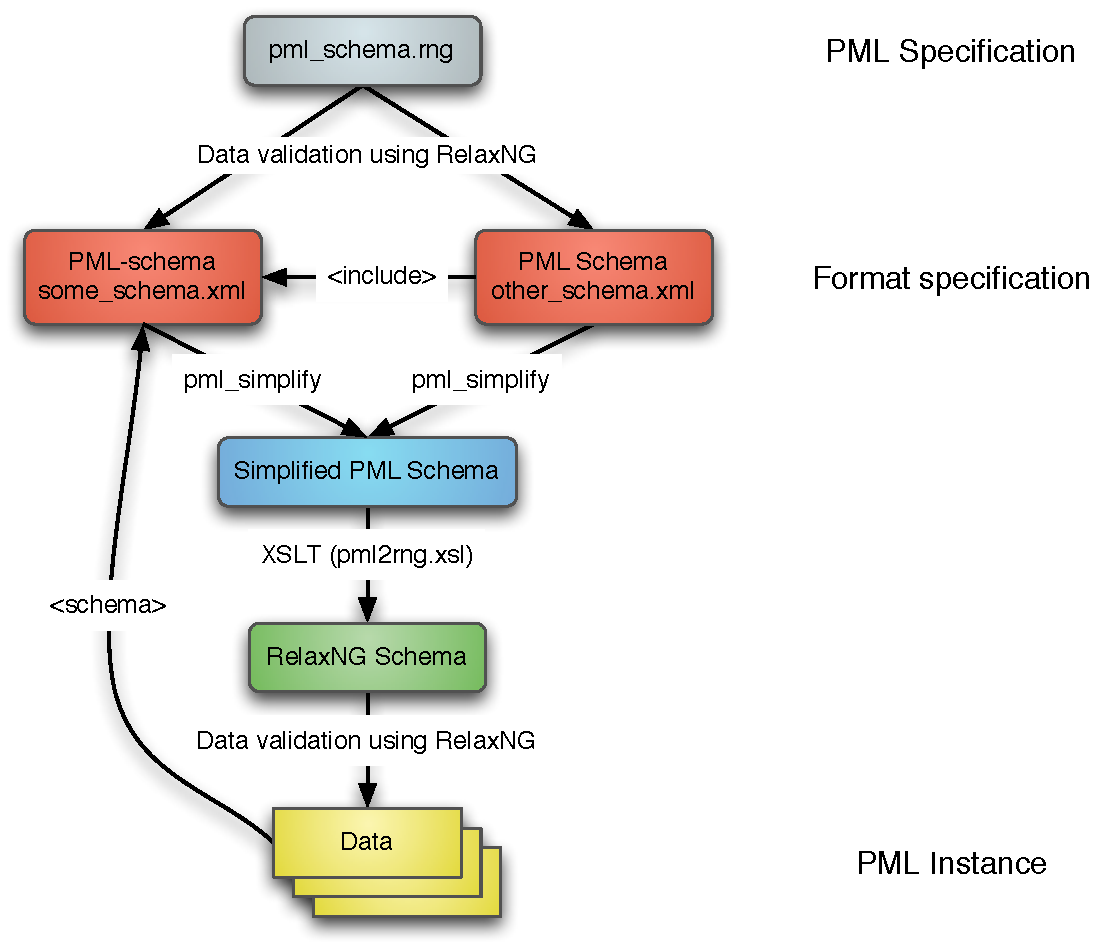
\includegraphics[width=\textwidth]{images/pml-schema.pdf}
   \caption{A schema of a PML workflow. It does not illustrate all the possible interactions of PML data and schema files.}
   \label{fig:pml}
\end{figure}

\section{Visualisation}
There are two basic ways to view st-nodes: in \seman\ or in \tred. Both of these need to use the ``t-a-m-w-'' PDT files to display the sentence and/or the tree for each sentence and then they read the \stf\ to add the information about \stn{}s. The \stn{}s are displayed as colour boxes or bubbles over the words in a sentence or nodes in a tree in \seman\ or \tred\ respectively.

\subsection{Visualisation using \seman}
The visualisation of annotated files in \seman\ has the advantage of showing whole text with all the \mwe{}s clearly marked in a single glance. Integration of the SemLex browser is also beneficial, because it allows fast and convenient lookup of annotated \mwe{}s in \seman. Details of \seman\ interface are described in \Sref{sec:seman}. 

There are, however, also some drawbacks of this ``full plain text of an article'' approach: 

\section{\tred\ extension}
\tred\ has a powerful mechanism that allows it to be extended for new tasks. We developed an extension \texttt{pdt-t-st} that allows to see MWEs as graphically marked groups of tectogrammatical nodes. 

 Main features of the extension:
 \begin{itemize}
\item
Merges the \stf{}s into \tf{}s and allows to display these enriched tectogrammatical trees.
\item
Types of annotated MWEs (i.e. types of NEs and \semlex\ entries) are distinguished with the same colours that were used in \seman\ during annotations. This allows not only for easily seeing NE types, but also easily spotting annotators' disagreement on them. 
\item
Allows to merge annotations of several annotators into one \tf. 
\item
Each annotator's MWEs have a unique raster. It is thus easy to spot annotators' partial or full disagreement not on types of MWEs, but also on their spans.
\end{itemize}

 There are two ways to merge the \sdata\ and \tdata: 
 \begin{enumerate}
\item
Merge on opening the \stf\ in \tred, and
\item
Static merge that produces the merged \verb=*.t.mwe.gz= file. 
\end{enumerate}
The dynamic merging is done using a newly developed feature of \tred\footnote{Developed by Petr Pajas} that allows to apply arbitrary perl transformations on the input data. Thus we open the \stf, use the mechanism of extensions to activate our extension by identifying the \stf\ as data the extension can process and call our transformation. The transformation requires a \tf\ annotated by this \sf\ to be present in the same directory. The \tf\ and \sf\ are parsed, and for each \stn\ we find a tectogrammatical tree that includes \tn{}s annotated (i.e. referenced) in this \stn. When we have a root of the correct t-tree, the \stn{}s are basically added into an attribute \texttt{mwes} of this t-root. The attribute is rather complex, because it contains lists of \stn{}s for all annotators that annotated any \stn{}s in this tree. Some small transformations of \stn{}s are needed, as well as creation of some new XML nodes, to represent the information from \sf{}s in the \tf{}s properly. For all the details inspect the code of \verb=<tred-extensions-dir>/pdt_t_st/libs/SDataMerge.pm=.